\documentclass[tikz,border=1.35mm]{standalone}

\definecolor{fvmadaptedge}{HTML}{8A7E7E}
\usetikzlibrary{arrows.meta}

\definecolor{externalface}{HTML}{8FB9E8}
\definecolor{splitred}{HTML}{AF2525}

% Static hexahedron anisotropic split scaffold.
% The wrapper files set \fvmadaptHexSplitCode before inputting this template.
\providecommand{\fvmadaptHexSplitCode}{1}

\newif\ifsplitxi
\newif\ifspliteta
\newif\ifsplitzeta
\ifnum\fvmadaptHexSplitCode>3
  \splitxitrue
\fi
\pgfmathtruncatemacro{\fvmadaptEtaMask}{mod(\fvmadaptHexSplitCode,4)}
\ifnum\fvmadaptEtaMask>1
  \splitetatrue
\fi
\pgfmathtruncatemacro{\fvmadaptZetaMask}{mod(\fvmadaptHexSplitCode,2)}
\ifnum\fvmadaptZetaMask=1
  \splitzetatrue
\fi

\begin{document}
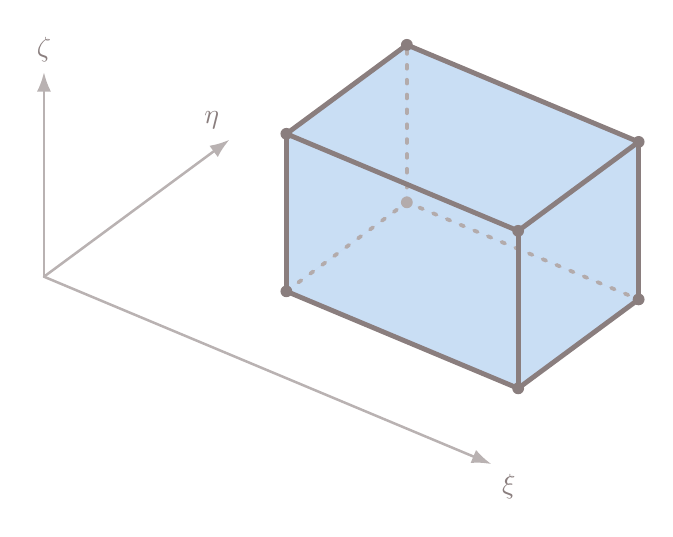
\begin{tikzpicture}[
  x={(20.3mm,-8.5mm)},
  y={(15.3mm,11.3mm)},
  z={(0mm,20mm)},
  line join=round,
  line cap=round,
  outer/.style={draw=fvmadaptedge,line width=0.62mm},
  hidden/.style={draw=fvmadaptedge!65,line width=0.48mm,loosely dotted},
  split/.style={draw=splitred,line width=0.50mm},
  face/.style={fill=externalface,fill opacity=0.28,draw=none},
  axis/.style={draw=fvmadaptedge!60,line width=0.32mm,-{Latex[length=2.5mm,width=1.8mm]}}
]
  % Parent hexahedron vertices. The xi direction is stretched to match the
  % other volume-cell figures.
  \coordinate (A) at (0,0,0);
  \coordinate (B) at (1.45,0,0);
  \coordinate (C) at (1.45,1,0);
  \coordinate (D) at (0,1,0);
  \coordinate (E) at (0,0,1);
  \coordinate (F) at (1.45,0,1);
  \coordinate (G) at (1.45,1,1);
  \coordinate (H) at (0,1,1);

  % Mid-plane coordinates used by the bitmask split codes.
  \coordinate (X00) at (0.725,0,0);
  \coordinate (X10) at (0.725,1,0);
  \coordinate (X11) at (0.725,1,1);
  \coordinate (X01) at (0.725,0,1);
  \coordinate (Y00) at (0,0.5,0);
  \coordinate (Y10) at (1.45,0.5,0);
  \coordinate (Y11) at (1.45,0.5,1);
  \coordinate (Y01) at (0,0.5,1);
  \coordinate (Z00) at (0,0,0.5);
  \coordinate (Z10) at (1.45,0,0.5);
  \coordinate (Z11) at (1.45,1,0.5);
  \coordinate (Z01) at (0,1,0.5);

  % Offset computational-coordinate axes.
  \coordinate (Oaxis) at (-1.20,-0.42,-0.18);
  \draw[axis] (Oaxis) -- (1.60,-0.42,-0.18) node[below right,font=\normalsize,text=fvmadaptedge] {$\xi$};
  \draw[axis] (Oaxis) -- (-1.20,1.12,-0.18) node[above left,font=\normalsize,text=fvmadaptedge] {$\eta$};
  \draw[axis] (Oaxis) -- (-1.20,-0.42,1.12) node[above,font=\normalsize,text=fvmadaptedge] {$\zeta$};

  % Exterior faces share the same translucent shade.
  \path[face] (A) -- (B) -- (C) -- (D) -- cycle;
  \path[face] (E) -- (F) -- (G) -- (H) -- cycle;
  \path[face] (A) -- (B) -- (F) -- (E) -- cycle;
  \path[face] (B) -- (C) -- (G) -- (F) -- cycle;
  \path[face] (C) -- (D) -- (H) -- (G) -- cycle;
  \path[face] (D) -- (A) -- (E) -- (H) -- cycle;

  % Draw split planes before the exterior wireframe so visible cell edges stay
  % visually dominant.
  \ifsplitxi
    \draw[split] (X00) -- (X10) -- (X11) -- (X01) -- cycle;
    \foreach \p in {X00,X10,X11,X01} {
      \fill[splitred] (\p) circle[radius=0.58mm];
    }
  \fi
  \ifspliteta
    \draw[split] (Y00) -- (Y10) -- (Y11) -- (Y01) -- cycle;
    \foreach \p in {Y00,Y10,Y11,Y01} {
      \fill[splitred] (\p) circle[radius=0.58mm];
    }
  \fi
  \ifsplitzeta
    \draw[split] (Z00) -- (Z10) -- (Z11) -- (Z01) -- cycle;
    \foreach \p in {Z00,Z10,Z11,Z01} {
      \fill[splitred] (\p) circle[radius=0.58mm];
    }
  \fi

  % Hidden-line convention: edges incident to the lower back-left vertex are
  % dotted.
  \draw[hidden] (A) -- (D) -- (C);
  \draw[hidden] (D) -- (H);

  % Visible exterior wireframe.
  \draw[outer] (A) -- (B) -- (C);
  \draw[outer] (E) -- (F) -- (G) -- (H) -- cycle;
  \draw[outer] (A) -- (E);
  \draw[outer] (B) -- (F);
  \draw[outer] (C) -- (G);

  % Original vertices are #8a7e7e, except the hidden lower back-left vertex D.
  \foreach \p in {A,B,C,E,F,G,H} {
    \fill[fvmadaptedge] (\p) circle[radius=0.75mm];
  }
  \fill[fvmadaptedge!65] (D) circle[radius=0.75mm];
\end{tikzpicture}
\end{document}
